%%%%%%%%%%%%%%%%%%%%%%%%%%%%%%%%%%%%%%%%%
% Jacobs Landscape Poster
% LaTeX Template
% Version 1.1 (14/06/14)
%
% Created by:
% Computational Physics and Biophysics Group, Jacobs University
% https://teamwork.jacobs-university.de:8443/confluence/display/CoPandBiG/LaTeX+Poster
% 
% Further modified by:
% Nathaniel Johnston (nathaniel@njohnston.ca)
%
% This template has been downloaded from:
% http://www.LaTeXTemplates.com
%
% License:
% CC BY-NC-SA 3.0 (http://creativecommons.org/licenses/by-nc-sa/3.0/)
%
%%%%%%%%%%%%%%%%%%%%%%%%%%%%%%%%%%%%%%%%%

%----------------------------------------------------------------------------------------
%	PACKAGES AND OTHER DOCUMENT CONFIGURATIONS
%----------------------------------------------------------------------------------------

\documentclass[final]{beamer}

\usepackage[scale=1.24]{beamerposter} % Use the beamerposter package for laying out the poster

\usepackage[utf8]{inputenc}

\usetheme{confposter} % Use the confposter theme supplied with this template

\setbeamercolor{block title}{fg=ngreen,bg=white} % Colors of the block titles
\setbeamercolor{block body}{fg=black,bg=white} % Colors of the body of blocks
\setbeamercolor{block alerted title}{fg=black,bg=dblue!70} % Colors of the highlighted block titles
\setbeamercolor{block alerted body}{fg=black,bg=dblue!10} % Colors of the body of highlighted blocks
% Many more colors are available for use in beamerthemeconfposter.sty

%-----------------------------------------------------------
% Define the column widths and overall poster size
% To set effective sepwid, onecolwid and twocolwid values, first choose how many columns you want and how much separation you want between columns
% In this template, the separation width chosen is 0.024 of the paper width and a 4-column layout
% onecolwid should therefore be (1-(# of columns+1)*sepwid)/# of columns e.g. (1-(4+1)*0.024)/4 = 0.22
% Set twocolwid to be (2*onecolwid)+sepwid = 0.464
% Set threecolwid to be (3*onecolwid)+2*sepwid = 0.708

\newlength{\sepwid}
\newlength{\onecolwid}
\newlength{\twocolwid}
\newlength{\threecolwid}
\setlength{\paperwidth}{48in} % A0 width: 46.8in
\setlength{\paperheight}{36in} % A0 height: 33.1in
\setlength{\sepwid}{0.024\paperwidth} % Separation width (white space) between columns
\setlength{\onecolwid}{0.22\paperwidth} % Width of one column
\setlength{\twocolwid}{0.464\paperwidth} % Width of two columns
\setlength{\threecolwid}{0.708\paperwidth} % Width of three columns
\setlength{\topmargin}{-0.5in} % Reduce the top margin size
%-----------------------------------------------------------

\usepackage{graphicx}  % Required for including images

\usepackage{booktabs} % Top and bottom rules for tables

%----------------------------------------------------------------------------------------
%	TITLE SECTION 
%----------------------------------------------------------------------------------------

\title{Bayesian network inference with simple propagation} % Poster title

\author{David Quesada López} % Author(s)

\institute{Computational Intelligence Group, Departamento de Inteligencia Artificial, Universidad Polit\'ecnica de Madrid, Spain} % Institution(s)

%----------------------------------------------------------------------------------------

\begin{document}

\addtobeamertemplate{block end}{}{\vspace*{2ex}} % White space under blocks
\addtobeamertemplate{block alerted end}{}{\vspace*{2ex}} % White space under highlighted (alert) blocks

\setlength{\belowcaptionskip}{2ex} % White space under figures
\setlength\belowdisplayshortskip{2ex} % White space under equations

\begin{frame}[t] % The whole poster is enclosed in one beamer frame

\begin{columns}[t] % The whole poster consists of three major columns, the second of which is split into two columns twice - the [t] option aligns each column's content to the top

\begin{column}{\sepwid}\end{column} % Empty spacer column

\begin{column}{\onecolwid} % The first column

%----------------------------------------------------------------------------------------
%	OBJECTIVES
%----------------------------------------------------------------------------------------

\begin{alertblock}{Objectives}

We propose \textit{simple propagation}, a new algorithm for tree propagation in exact inference in discrete bayesian networks. It aims to:
\begin{itemize}
\item Outperform lazy propagation in terms of efficiency.

\item Have a good performance in optimal join trees. 

\end{itemize}

\end{alertblock}

%----------------------------------------------------------------------------------------
%	INTRODUCTION
%----------------------------------------------------------------------------------------

\begin{block}{Introduction}

Exact inference is a method used to answer queries asked to bayesian networks. One of the ways to go around exact inference is through jion trees. This trees are built from the DAG, and tipically at each node of the tree a potencial is computed by multiplying the probability tables inside it.

\begin{itemize}

\item Lazy propagation (LP) \cite{madsen1999} keeps a multiplicative factorization of potentials at each node. This helps to identify irrelevant potencials at the moment of sending a message from a node. When it identifies the relevant potencials, LP builds a graph to determine elimination ordering of the variables.

\item Simple propagation (SP) uses a "one in, one out" property at the moment of sending a message from a node to eliminate variables. This way, it works greedily towards the elimination of variables, not needing to build a graph to determine the elimination order

\end{itemize}


\end{block}

%------------------------------------------------


%----------------------------------------------------------------------------------------

\end{column} % End of the first column

\begin{column}{\sepwid}\end{column} % Empty spacer column

\begin{column}{\twocolwid} % Begin a column which is two columns wide (column 2)

\begin{columns}[t,totalwidth=\twocolwid] % Split up the two columns wide column

\begin{column}{\onecolwid}\vspace{-.6in} % The first column within column 2 (column 2.1)

%----------------------------------------------------------------------------------------
%	MATERIALS
%----------------------------------------------------------------------------------------

\begin{block}{Materials}

To conduct a comparison between the performance of LP and SP we used 28 benchmark bayesian networks. Then we generate 100 sets of evidence randomly and compute the message passing to calculate the posterior probabilities given the evidence for each non-evidence variable. Finally, we compare the average results in computation time of LP and SP.


\end{block}

\begin{alertblock}{Only for optimal join trees}

Simple propagation performance significantly degrades in non-optimal join trees. 

\end{alertblock} 

\begin{figure}
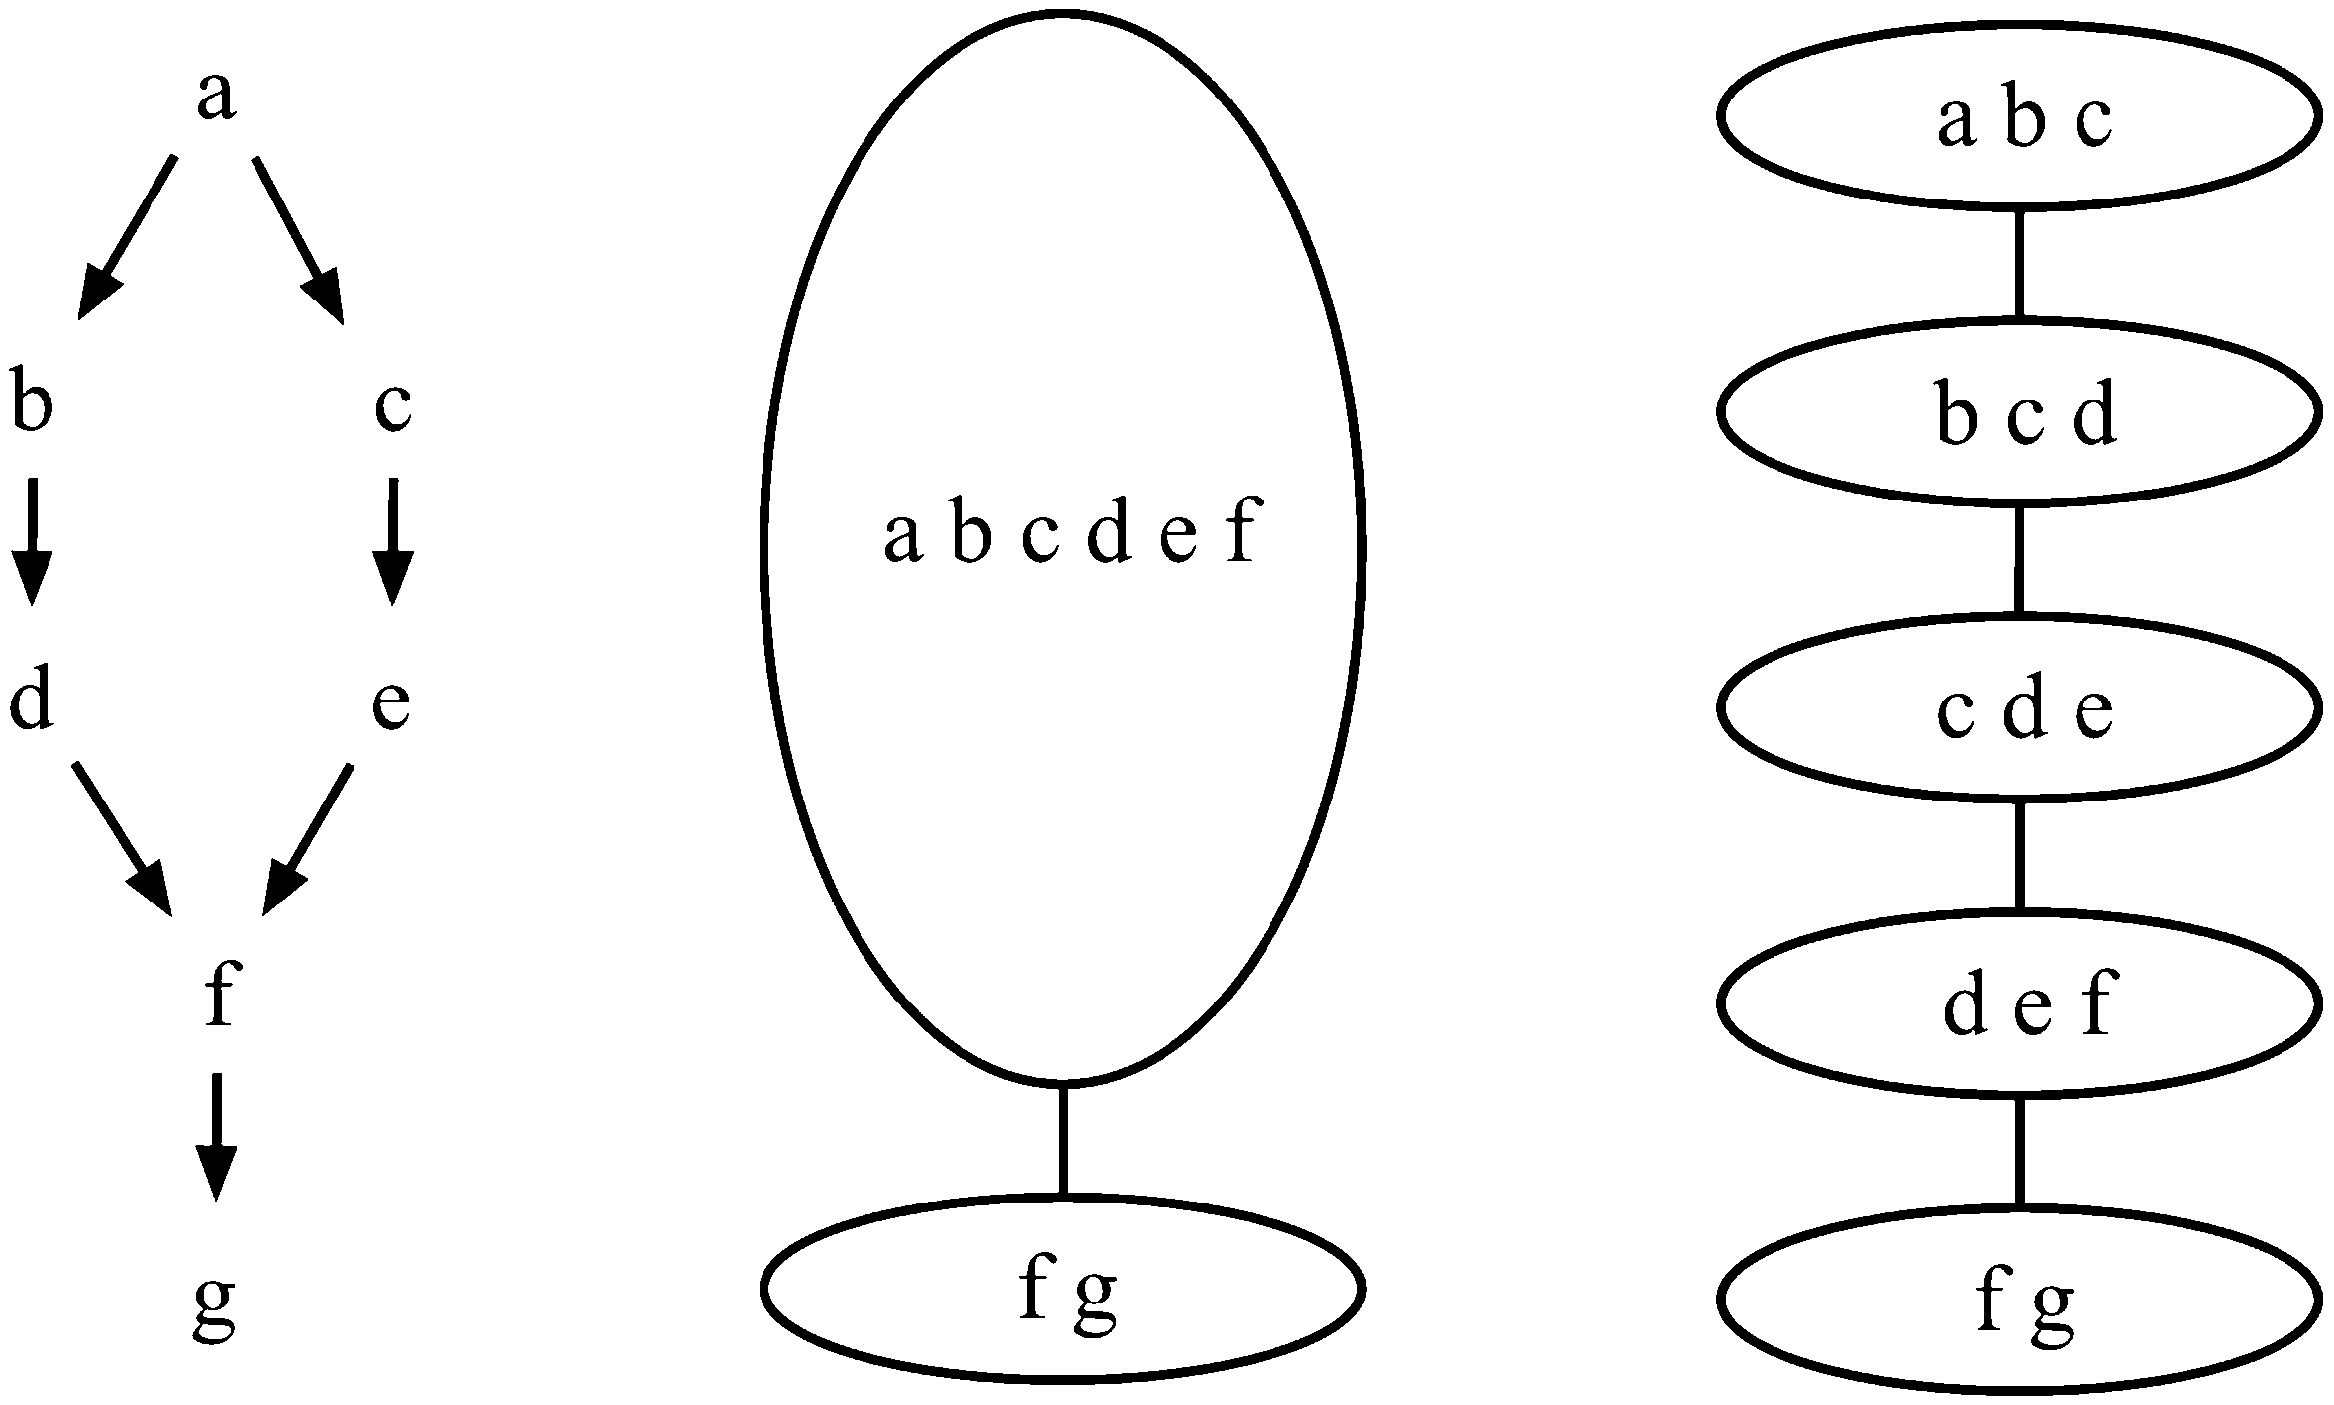
\includegraphics[width=0.8\linewidth]{optimal.png}
\caption{Non-optimal and optimal join trees of a BN}
\end{figure}

\begin{block}{One in, one out}

When a node N is ready to construct its message to a neighbour sharing
variables S, SP recursively identifies those potentials at N with a “one in, one out” property, namely,
the potential has at least one non-evidence variable in S and another not in S. SP then eliminates
each “out” variable. SP is often faster than LP in experimental results involving optimal (or close
to) join trees built from numerous real-world and benchmark BNs (Butz et al., 2016)

By “one in, one out”, we mean a
potential in F has at least one non-evidence variable in the separator and another non-evidence
variable not in the separator.



\end{block}

%----------------------------------------------------------------------------------------

\end{column} % End of column 2.1

\begin{column}{\onecolwid}\vspace{-.6in} % The second column within column 2 (column 2.2)

%----------------------------------------------------------------------------------------
%	Heuristics
%----------------------------------------------------------------------------------------

\begin{block}{Heuristics proposed}

We propose some heuristics to select the order in wich we evaluate potentials satisfying the “one in, one out” property based on:

\begin{itemize}

\item Increasing number of variables in X.
\item Decreasing number of variables in X.
\item Increasing number of variables of both X and S.
\item Decreasing number of variables of both X and S.

\end{itemize}

\end{block}

\begin{block}{Results}

Our study shows that SP is faster than LP in 18 cases, equal in 5 cases and slower in 5 cases. When SP is slower, further research showed that it is because LP has more elimination orderings to choose from, and when it is considerably better than the one SP uses, it is faster even though it spent more time building graphs to determine this ordering. This is also the case why LP is better for non-optimal join trees.

\begin{table}
\vspace{2ex}
\begin{tabular}{l l l}
\toprule
\textbf{Heuristic} & \textbf{Wins} \\
\midrule
Arbitrary & 6 \\
Increasing X & 1 \\
Decreasing size S & 1 \\
\bottomrule
\end{tabular}
\caption{Heuristic selection results}
\end{table}

We also tried our heuristics in selecting the order of evaluation of potencials: out of 29 BNs, heuristic and arbitrary order tied in 13 cases, arbitrary won in 6 and heuristic won in 2. This means that the selection of the order is not really relevant to SP.

\end{block}

%----------------------------------------------------------------------------------------

\end{column} % End of column 2.2

\end{columns} % End of the split of column 2 - any content after this will now take up 2 columns width

%----------------------------------------------------------------------------------------
%	Optimal join trees
%----------------------------------------------------------------------------------------



%----------------------------------------------------------------------------------------

\begin{columns}[t,totalwidth=\twocolwid] % Split up the two columns wide column again


\end{columns} % End of the split of column 2

\end{column} % End of the second column

\begin{column}{\sepwid}\end{column} % Empty spacer column

\begin{column}{\onecolwid} % The third column

%----------------------------------------------------------------------------------------
%	CONCLUSION
%----------------------------------------------------------------------------------------

\begin{block}{Conclusion}

\begin{itemize}
\item Simple propagation for exact inference performs in general better than lazy propagation when provided with an optimal join tree.
\item It's performance doesn't seem to improve even with our proposed heuristics in optimal or non-optimal join trees. 
\item It is still an exact inference method, so its use is restricted to tractable bayesian networks.
\end{itemize}
 

\end{block}

%----------------------------------------------------------------------------------------
%	Artículo real
%----------------------------------------------------------------------------------------

\begin{block}{Artículo real}

Butz C. J., Oliveira J. S., dos Santos A. E., Madsen, A. L. (2018). An empirical study of Bayesian network inference with simple propagation. \textit{International Journal of Approximate Reasoning}, 92, 198-211.

\end{block}

%----------------------------------------------------------------------------------------
%	Referencias
%----------------------------------------------------------------------------------------

%\setbeamercolor{block title}{fg=red,bg=white} % Change the block title color

\begin{block}{Referencias}
\nocite{*} % Insert publications even if they are not cited in the poster
\small{\bibliographystyle{plainnat}
\bibliography{sample}\vspace{0.75in}}
\begin{thebibliography}{}

\bibitem{madsen1999}
A.L. Madsen, F.V. Jensen, Lazy propagation: a junction tree inference algorithm based on lazy evaluation, Artif. Intell. 113 (1–2) (1999) 203–245

\end{thebibliography}


\end{block}

%----------------------------------------------------------------------------------------
%	CONTACT INFORMATION
%----------------------------------------------------------------------------------------

%\setbeamercolor{block alerted title}{fg=black,bg=norange} % Change the alert block title colors
%\setbeamercolor{block alerted body}{fg=black,bg=white} % Change the alert block body colors

\begin{center}
\begin{tabular}{ccc}

\includegraphics[width=0.4\linewidth]{logoUPM.jpg} 
\end{tabular}
\end{center}

%----------------------------------------------------------------------------------------

\end{column} % End of the third column

\end{columns} % End of all the columns in the poster

\end{frame} % End of the enclosing frame

\end{document}
